\begin{table}[t!]
\small
  \centering
    \begin{tabular*}{0.48\textwidth}{l|c|c|c|c}
    \hline
    Method                & Input Data  & Shapes & Classes & Acc         \\
    \hline
    \hline
    \protect\cite{Huang:2013:FSL} & 3D Warehouse & 1206-5850 & 26 & 86 \\
    \protect\cite{Golovinskiy:2009:SBR3D} & LIDAR & 1063  & 16 & 58  \\
    \protect\cite{Shilane:2007:drs} & PSB & 1814 & 90 & 75 \\
    \protect\cite{Funkhouser:2006:pm3d} & PSB & 1814 & 90 & 83 \\
    \protect\cite{Barutcuoglu:2006:hscu} & PSB & 1814 & 90 & 84 \\
    \protect\cite{Bronstein:2011:SGGW} & SG & 715 & 13 & 89 \\
    \protect\cite{Litman:2014:SLBF} & SG & 715 & 13 & 91 \\
    \protect\cite{Li:2012:SHREC} & SHREC12 & 1200 & 60 & 88 \\
     \protect\cite{Li:2014:SHREC} & SHREC14 & 400-$10^4$ & 1352 & 87\\
    \protect\cite{Wu:3SN:2015} & ModelNet40 & 48,000 & 40 & 77 \\
     \protect\cite{Su:MCN:2015} & ModelNet40 & 48,000 & 40 & 90\\
     \protect\cite{Su:2016aa} & ModelNet40 & 48,000 & 40 & 94 \\
%    \hline
%    \multicolumn{5}{c}{Nearest neighbor classifier with different shape descriptors} \\
%    \hline 
%    \cite{Chaudhuri:2013:ACC} & supervised     & pairwise comparison  & meshes (parts) & 42-100 & 7-14 & N/A \\
    \hline
    \end{tabular*}
  \caption{\rev{Performance of several methods for shape classification (the accuracy in the right-most column as measured as fraction of correctly-labeled shapes). Huang et al.~\protect\cite{Huang:2013:FSL}
predict fine-grained tag attributes for big collections of similar shapes. Golovinskiy et al.~\protect\cite{Golovinskiy:2009:SBR3D}
propose a method for classifying point clouds of objects in urban environments. The methods aimed at classifying meshes are evaluated on Princeton Shape Benchmark (PSB)~\protect\cite{Shilane:2007:drs,Funkhouser:2006:pm3d,Barutcuoglu:2006:hscu}. To evaluate performance of the method in the presence of non-rigid deformations ShapeGoogle (SG) dataset is also commonly used~\protect\cite{Bronstein:2011:SGGW,Litman:2014:SLBF}.
%In addition several methods can be found in regular shape retrieval challenges~\protect\cite{Li:2012:SHREC,Li:2014:SHREC}. 
\revnew{Several recent techniques use uniformly sampled representations (volumetric and view-based images) of 3D shapes in conjunction with neural networks~\protect\cite{Wu:3SN:2015,Su:MCN:2015,Su:2016aa}.}
} }
  \label{tab:classification_performance}
\end{table}




\begin{figure}[bt]
\centering
    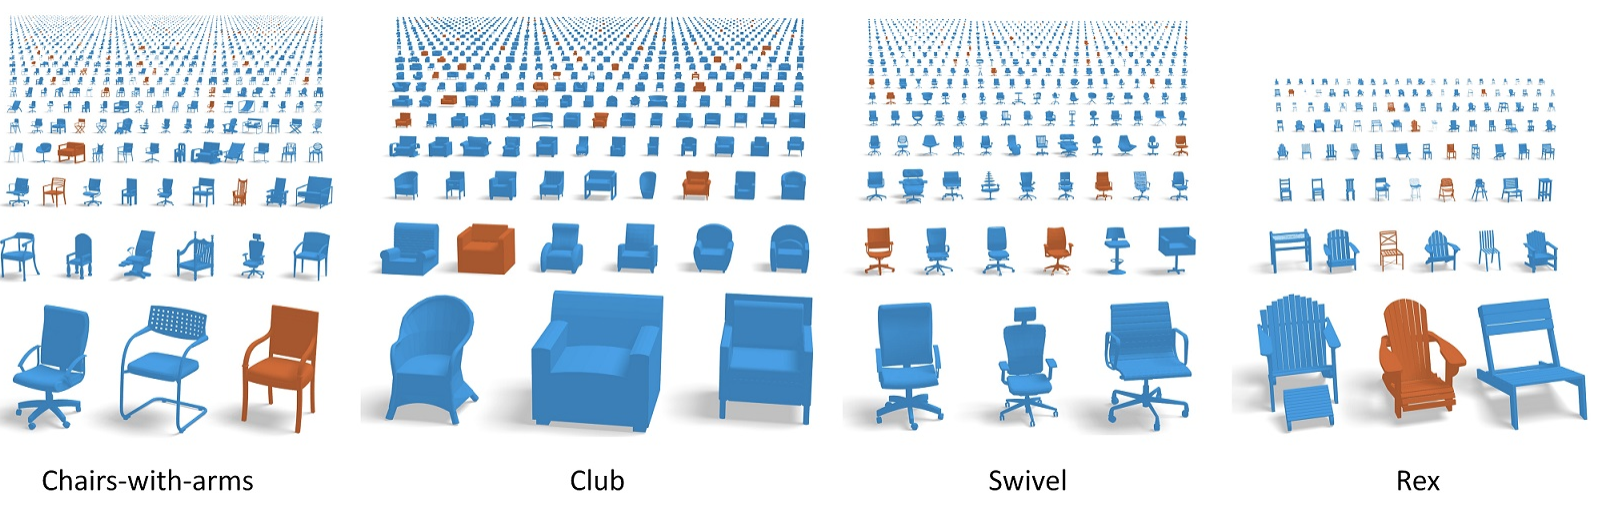
\includegraphics[width=1.0\columnwidth]{fig/search/huang_siga13_fine.png}
   %\vspace{-.6cm}
    \caption{
    Fine-grained classification of 3D models \cite{Huang:2013:FSL}, where text labels are propagated from brown to blue models. }
    \label{fig:fine-grained}
\end{figure}



\section{Shape classification}
\label{sec:classification}
% search / retrieval / classification
\rev{Data-driven techniques commonly make assumptions about the size and homogeneity of the input data set. In particular, existing analysis techniques often assume that all models belong to the same class of objects~\cite{Kim:2013:lpt} or scenes~\cite{Fisher:2011:CSR}, and cannot directly scale to entire repositories such as the Trimble 3D Warehouse~\cite{warehouse}. Similarly, techniques for data-driven reconstruction of indoor environments assume that the input data set only has furniture models~\cite{Nan:2012:SAC}, while modeling and synthesis interfaces restrict the input data to particular object or scene classes~\cite{Chaudhuri:2011:prabm,Kalogerakis:2012:PMC,Fisher:2012:CSR}.  Thus, as a first step these methods need to query a 3D model repository to retrieve a subset of relevant models.}

\rev{Most public shape repositories such as 3D Warehouse~\cite{warehouse} rely on the users to provide tags and names of the shapes with little additional quality control measures. As a result, the shapes are sparsely labeled with inconsistent and noisy tags.  This motivates developing automatic algorithms to infer text associated with models.  Existing work focuses on establishing class memberships for an entire shape (e.g. this shape is a chair), as well as inferring finer-scale attributes (e.g. this chair has a rocking leg).}


\rev{ \paragraph*{Classification} methods assign a class membership for unlabeled shapes. One approach is to retrieve for each unlabeled shape the most similar shape from a database of 3D models with known shape classes. There has been a large number of shape descriptors proposed in recent years that can be used in such a retrieval task, and one can refer to various surveys (e.g., \cite{Tangelder:2008:ASC}) for a thorough overview and comparisons. }
%
\rev{One can further improve classification results by leveraging machine learning techniques to learn classifiers that are based on global shape descriptors~\cite{Frome:2004:rord,Golovinskiy:2009:SBR3D}. Barutcuoglu et al.~\cite{Barutcuoglu:2006:hscu} demonstrate that Bayesian aggregation can be used to improve classification of shapes that are a part of a hierarchical ontology of objects. Geometry matching algorithms also facilitate distinguishing important features for classification~\cite{Funkhouser:2006:pm3d,Shilane:2007:drs}. Bronstein et al.\cite{Bronstein:2011:SGGW} leverage ``bag of features'' to learn powerful descriptor-space metrics for non-rigid shapes. These technique can be further improved by using sparse coding techniques~\cite{Litman:2014:SLBF}.  In recent shape retrieval challenges, techniques based on bag of features demonstrated the best performance~\cite{Li:2012:SHREC,Li:2014:SHREC} in comparison to other alternatives. See Table~\ref{tab:classification_performance} for a brief summary of some methods.}



% todo: figure for chaudhuri, for huang

\paragraph*{Tag attributes} often capture fine-scale attributes of shapes that belong to the same class.
These attributes can include presence or absence of particular parts, object style, or comparative adjectives.
%
Huang et al.~\cite{Huang:2013:FSL} developed a framework for propagating these attributes in a collection of partially annotated 3D models. For example, only brown models in Figure \ref{fig:fine-grained} were labeled, and blue models were annotated automatically. To achieve automatic labeling, they start by co-aligning all models to a canonical domain, and generate a voxel grid around the co-aligned models. For each voxel they compute local shape features, such as spin images, for each shape. Then, they learn a distance metric that best discriminates between different tags. All shapes are finally embedded in a weighted feature space where nearest neighbors are connected in a graph. A graph cut clustering is used to assign tags to unlabeled shapes.
%
\fix{Tag attributes can also be used to describe semantics, function, or style of parts in shapes. Data-driven consistent segmentation and labeling techniques can be applied to propagate part tags across shapes (see Section \ref{sec:segmentation}). An alternative approach is to partition shapes into multiple sets of parts, then extract descriptors to define part similarity. A characteristic example of such an approach was demonstrated in Shapira et al.~\cite{Shapira:2010:CPA}. Given the hierarchical segmentations of 3D shapes as input, part tagging was achieved by comparing local geometric features of parts as well as their context within the whole shape.}
%\fix{
%With hierarchical segmentation of 3D objects as input,
%Shapira et al.~\cite{Shapira:2010:CPA} propose contextual part analogies to achieve part tagging.
%To establish part-level correspondence among different 3D objects, a context enhanced part-in-whole matching where
%part similarity is measured based not only on local geometric signatures but also on their context within the whole shape.
%With such part analogies, textual tags of object parts can be carried from one model to others.
%}

\rev{ While the above method works well for discrete tags, they do not capture more continuous relations, such as animal A is more dangerous than animal B.  Chaudhuri et al.~\cite{Chaudhuri:2013:ACC} focus on estimating ranking based on comparative adjectives. They use crowdsourcing to gather pairwise comparisons of shape parts with respect to different adjectives, and use a Support Vector Machine ranking method to predict attribute strengths from shape features for novel shape parts (Figure \ref{fig:attribit}). }

\begin{figure}[tb]
\centering
    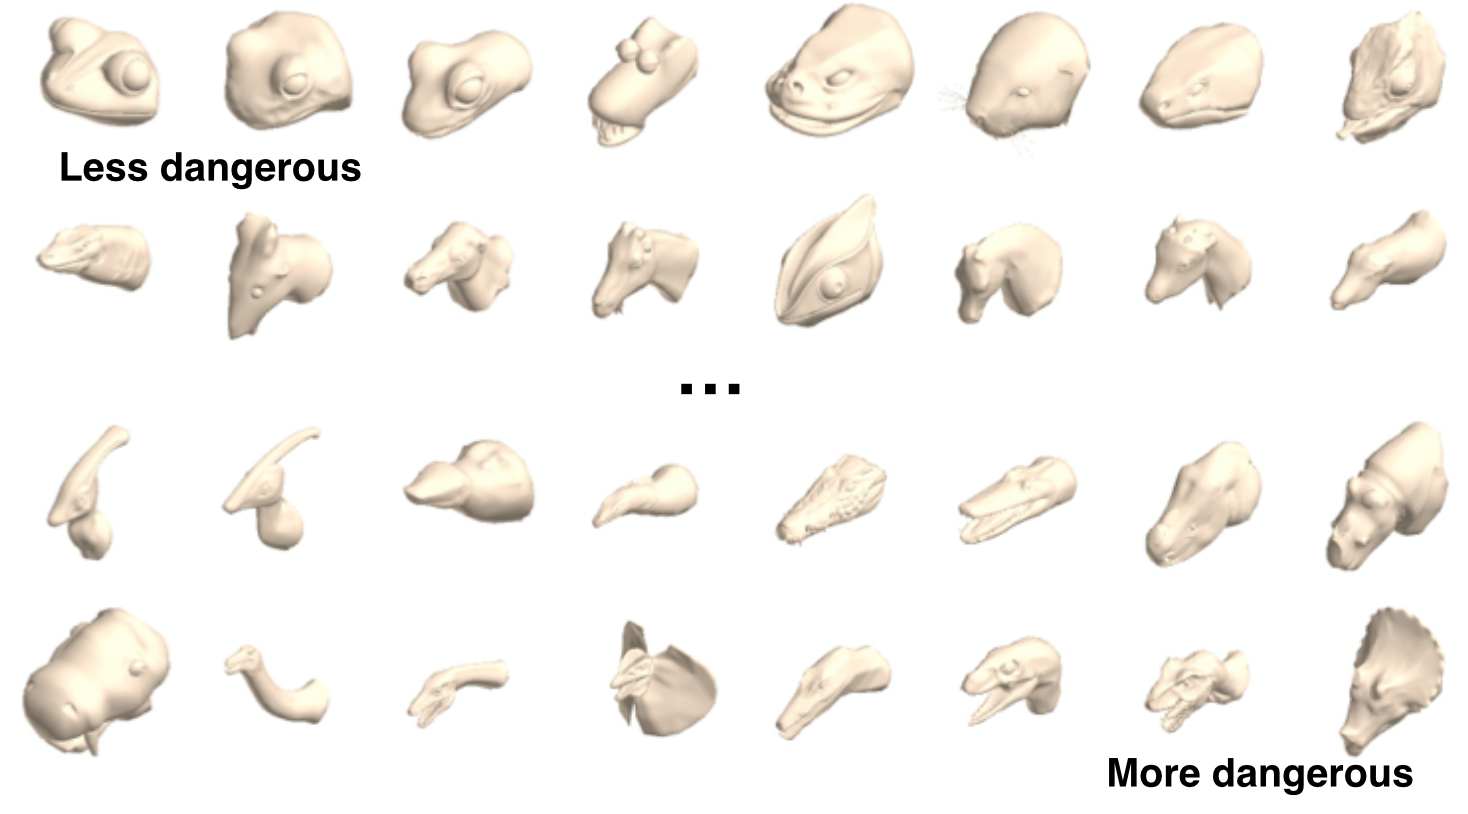
\includegraphics[width=1.0\columnwidth]{fig/search/chaudhuri_uist13_attr.png}
    %\vspace{-.6cm}
    \caption{
    Ranking of parts with respect to ``dangerous'' attribute (image from \cite{Chaudhuri:2013:ACC}) }
    \label{fig:attribit}
\end{figure}



\rev{ \paragraph*{Style similarity} methods have recently been proposed to classify shapes into style-related categories e.g., buildings can be classified into architectural styles, such as Gothic, Baroque, Byzantine and so on. In contrast to the previously discussed approaches that rely on generic visual similarity measures to compare shapes, these methods learn distance functions for style elements \cite{lun:style:2015} or common feature spaces \cite{liu:style:2015} to quantify the stylistic similarity of shapes. The methods can be used to compare the style similarity of shapes, even when these belong to different classes (e.g., chairs and lamps). To align the style similarity measures with the human perception of style, style comparisons of shapes are gathered through crowdsourcing.  The learned similarity measures can be used to retrieve stylistically similar shapes to populate a scene, or associate shapes with style-related tags. }

% limitations
%While the techniques described above are suitable for retrieving related models, most of the described method are not designed to understand intra-class variations. Usually a more involved structural analysis is necessary to understand higher-level semantic properties of shapes. Even for inferring tag attributes existing works relies on shape matching~\cite{Huang:2013:FSL} or shape segmentation~\cite{Chaudhuri:2013:ACC}. The following two sections will focus on inferring these higher-level structural properties in collections of shapes.

\rev{ While the techniques described above are suitable for retrieving and classifying shapes, a large number of applications require a more involved structural analysis to infer semantic and functional properties of shapes or their parts. The following two sections will discuss methods that perform structural analysis in collections of shapes based on segmentation and local matching.}

